\chapter{EJB}
\label{EJB}
\thispagestyle{chapternohead}

	
\pagestyle{ruledfilip}

\section{What is EJB?}

\begin{itemize}
	\item EJB is just a specification. It is not a product.
	\item An EJB is just a collection of Java classes and XML file,
	bundled into a single unit. The Java classes must follow
	certain rules.
	\item EJBs are reusable components.
	\item EJB is a widely-adopted server-side component architecture
	for J2EE.
	\item EJB components are designed to encapsulate business logic,
	and to protect the application developer from having to
	worry about system level issues.
\end{itemize}

\section{Key features of EJB}

\begin{itemize}
	\item EJB components are server-side components written entirely in Java
	\item EJB components contain business logic only
	\item System-level services (i.e. "plumbing") such as transactions,
	security, Life-cycle, threading, persistence, etc. are
	automatically managed for the EJB component by the EJB
	server
	\item EJB components are fully portable across any EJB server
	and any OS, work with any client.
\end{itemize}

\section{EJB vs JavaBeans}

\begin{itemize}
	\item The JavaBeans architecture is meant to provide a format for
	general-purpose components whereas the EJB architecture
	provides a format for encapsulation and management of
	business logic.
	\item JavaBeans has tier of execution at Client and EJB has at
	Server (specifically business logic tier)
	\item In JavaBeans the runtime execution environment provides
	services like Java libraries, Java application etc.
	\item The EJB runtime environment provides services of
	persistence, declarative transactions and security, connection
	pooling and lifecycle services.
\end{itemize}

 
\begin{figure}[tbph!]
	\centering
	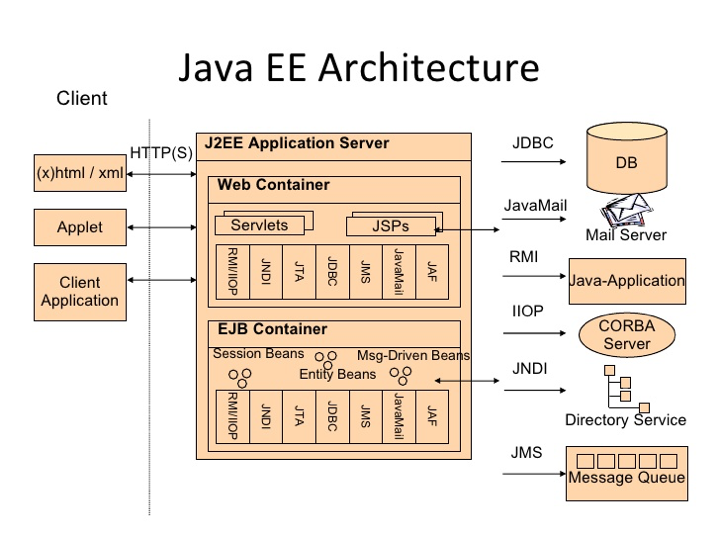
\includegraphics[width=0.7\linewidth]{images/javaeearchitecture}
	\caption{}
	\label{fig:javaeearchitecture}
\end{figure}

\section{Varieties of Beans}

\begin{itemize}
	\item Session Beans
	\begin{itemize}
		\item Store data of a particular client for the duration of his session
		\item types
		\begin{itemize}
		\item Stateful session bean
		\item Stateless session bean
		\item Singleton
		\end{itemize}
	\end{itemize}
	\item Entity Beans
	\begin{itemize}
		\item Persistent data storage (with container-managed persistence)
		\item With bean-managed persistence
	\end{itemize}
	\item Message-Driven Beans
\end{itemize}
\subsection{Session Beans}

\subsubsection{Stateless}
\begin{itemize}
	\item no conversational state between methods
	\item pool of multiple instances
\end{itemize}

\subsubsection{Stateful}

\begin{itemize}
	\item conversational state for a single user
	\item instance per session
\end{itemize}

\subsubsection{Singleton}

\begin{itemize}
	\item shared between clients
	\item only one instance exists for the entire application
\end{itemize}

\section{Roles in EJB Development}


\section{EJB Container and its Services}


\section{Services provided by an EJB container}


\section{How the Container Provides Services}


\section{Contracts}

\section{Local vs Remote}

\section{Interposition:	from remote client to EJB Container}

\section{Working with EJBs}

\section{Clients}

\section{The Client Developer’s View}

\section{EJB’s interface}


\section{The Bean Programmer’s view}


\section{EJB3 example}

AppleManagement Interface

\begin{minted}{java}
import java.rmi.RemoteException;


@Remote
public interface AppleManagement {
	public List<Apple> grabApples(AppleTree tree, int quantity)
		throws RemoteException;
	public void biteApple(Apple apple) throws RemoteException;
	public boolean hasApples(AppleTree tree) throws RemoteException;
}
\end{minted}


\section{CDI vs EJB}



\section{Example EJB: the Timer service}



\section{Types of timers}





%%% Local Variables:
%%% mode: latex
%%% TeX-master: "masterproef"
%%% End:

